\documentclass[11pt,letterpaper]{article}

\usepackage[letterpaper,margin=0.8in,nohead]{geometry}

\usepackage[colorlinks]{hyperref}
\usepackage{url}
\usepackage{breakurl}

\hypersetup{
	colorlinks,
	linkcolor={red},
	citecolor={red},
	urlcolor={blue}
}

\usepackage{verbatim}
\usepackage{fancyvrb}
\usepackage{scrextend}
\usepackage{enumitem}
\usepackage{url}
\usepackage{subcaption}

\usepackage{filecontents}
%\usepackage{natbib}
%\nobibliography*

\usepackage{caption}
\usepackage{graphicx}

\usepackage{changepage}   % for the adjustwidth environment

\newenvironment{answer}{\em \color{blue} \begin{adjustwidth}{1cm}{1cm}}{\end{adjustwidth}}

% math
\usepackage{amsthm,amsmath}
\usepackage{amsfonts}
\usepackage{float}

\newcommand{\mc}[1]{\mathcal{#1}}	% Mechanisms / Algorithms
\newcommand{\rv}[1]{\mathbf{#1}}    % Random variable

\newcommand{\pr}[1]{\mathrm{Pr}\{#1\}} % Probability

\newtheorem{corollary}{\bf Corollary}%[theorem]
\newtheorem{lemma}{\bf Lemma}%[theorem]
\newtheorem{definition}{\bf Definition}%[section]

\newtheorem{observation}{\bf Observation}%[theorem]



% load cleveref last!
\usepackage[capitalise]{cleveref}

\crefname{observation}{Observation}{Observations}


\begin{document}
	
	\title{EN4720: Security in Cyber-Physical Systems \\ Programming Assignment --- Passwords}
	
	%% This is an individual assignment!!
	%% TODO: put your name and index number here here!
	\author{ \textcolor{blue}{Name: Thalagala B. P.} \\ \textcolor{blue}{Index No: 180631J}}
	
	\maketitle
	
	\begin{center}
		\color{red}\bf This is an individual assignment! \\ Due Date: 8 July 2023 by 11.59 PM
	\end{center}
	
	\begin{center}
		\small Content adopted from {\bf CNT5410 Computer and Network Security} taught by Prof. Vincent Bindschaedler at the University of Florida.
	\end{center}
	
	\section*{Instructions}
	%
	
	Please read the instructions and questions carefully. Write your answers directly in the space provided. Compile the tex document and hand in the resulting PDF as your report.
	
	In this assignment, you will write a few lines Python code. You are encouraged to use Python3. You will need the PyCrypto library to run the provided code. Please refer to resources specific to your operating system and environment for installation instructions\footnote{\url{https://pypi.org/project/pycrypto/} See also:  \url{https://www.pycryptodome.org/en/latest/index.html}.}. For example, you can use: \texttt{pip3 install pycrypto} to install PyCrypto with Python3 under Linux.
	
	\subsection*{Assignment Files}
	The assignment archive contains the following Python source files:
	%
	\begin{itemize}[nolistsep]
		\item \texttt{utils.py}. This file contains utility functions needed for the assignment..
		\item \texttt{crypto.py}. This file defines cryptographic functions. 
		\item \texttt{attack.py}. This file contains attack code used in the assignment.
	\end{itemize}
	
	\noindent
	In addition, the assignment archive contains a \texttt{data} directory which includes a dictionary file (\texttt{words.list}) and several database dump files in JSON format (\texttt{*-dbdump.json}).
	
	\subsection*{Submission}
	Write your answers directly in the space provided. Compile the tex document and submit the resulting PDF together with the source code in a single zip file through Moodle.
	
	\bigskip
	
	\noindent
	\underline{Note:} \\
	\noindent You are encouraged to take a look at the provided files. This may help you successfully complete the assignment. \\
	\noindent 
	You might have to change the line ``from Cryptodome.Hash import SHA256'' in crypto.py to ``from Crypto.Hash import SHA256'' based on your OS and library versions. \\
	\noindent
	The program can take a while to run and the terminal might not show anything until program execution is complete. But it should not take more than 5 minutes (max).
	
	\newpage
	\section*{Problem 0: Bruteforce attack (12 pts)}
	%
	In this problem, you will mount a bruteforce attack against a stolen database dump of password hashes (\texttt{data/simple-dbdump.json}). The code for this problem is already written. (But you are encouraged to take a look to see how it works.)
	
	The bruteforce attack will try all possible passwords of 4 (or less) alphanumeric characters --- lowercase only. To perform the attack run the following command\footnote{You may have to specify to use Python3 \texttt{python3} if you also have Python2 versions installed on your system.}:
	%
	\begin{Verbatim}
		python attack.py problem0
	\end{Verbatim}
	%
	
	\begin{enumerate}
		
		\item (2 pts) What steps can you take to create a password that is hard to crack using bruteforce attacks?
		
		\begin{answer}
			
			\begin{itemize}
				\item A \textbf{combination of numbers, letters (upper case and/or lower case)  and special characters} must be used. This make the number of options per character to be large which eventually make it hard to brute-force.
				
				\item \textbf{The password must be sufficiently long}. This makes the number of possible password combinations (password space) extremely large which will make the brute-force attack computationally infeasible to be done in a shorter period of time. 
			\end{itemize}
			
		\end{answer}
		
		\item (4 pts) Which passwords are recovered (for which users)? How long did the attack take (in seconds)? What was the speed of the attack (in hashes/second)? Add a screenshot of your terminal output showing the answer.
				
		
		\begin{answer}
			
			\begin{figure}[h]
				\centering
				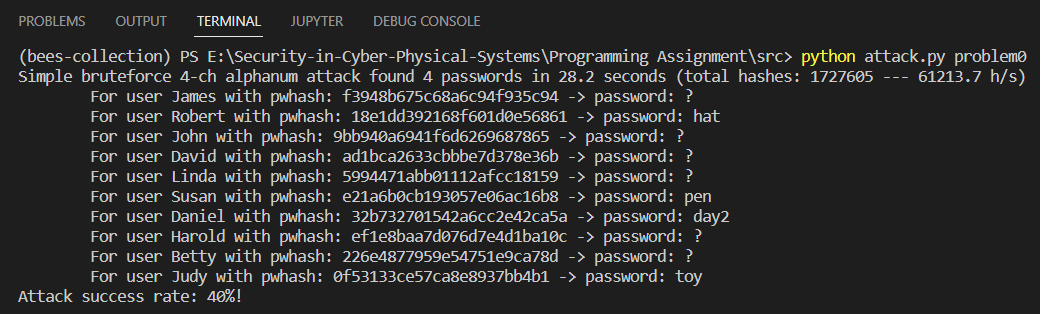
\includegraphics[width=0.8\columnwidth]{images/p0/q1.png}
				\caption{Output of the {\tt python attack.py problem0}}
			\end{figure}
			
			\begin{itemize}
				\item Time for the attack = 28.2 seconds
				\item Speed of the attack = 61213.7 hashes per second
				\item Attack success rate: 40\%				
			\end{itemize}
			
			\begin{table}[h]
				\centering
				\begin{tabular}{|l|l|}
					\hline
					\textbf{User} & \textbf{Password} \\ \hline
					Robert & hat \\ \hline
					Susan & pen \\ \hline
					Daniel & day2 \\ \hline
					Judy & toy \\ \hline
				\end{tabular}
				\caption{Recovered Passwords}
			\end{table}			
			
		\end{answer}
		\pagebreak
		\item (2 pts) What is the total number of {\em possible} passwords of $l$ {\em or less} alphanumeric characters --- lowercase only? 
		
		\begin{answer}
			
			Since there are 26 lowercase letters and 10 digits, there are a total of 36 possible characters that can be used in each position of the password. For a password of length $n$, there are $36^n$ passwords. If we consider the passwords of length l and less, we can have the following number of total passwords, which is the sum of a geometric series where number of terms equal to $l$, common ratio is 36 and the first term is 36.
			
			\begin{equation}
				\sum_{n=1}^{l} 36^n = 36 \cdot \frac{36^l -1}{36 - 1} = \frac{36^{l+1}-36}{35}
			\end{equation}
			
			In addition, the program considers an empty string ({\tt `'})  as the first candidate password. Therefore the total password count becomes,
			
			\[
				\frac{36^{l+1}-36}{35} + 1 = \frac{36^{l+1}-1}{35}
			\]			
			
		\end{answer}
		
		\item (4 pts) Given your previous answers. How long do you estimate it would take to perform the same attack on all passwords of $8$ or less alphanumeric characters --- lowercase only? (Justify your answer.) Can you confirm your calculation experimentally?
		
		\begin{answer}
			
			Total number of possible passwords say $P$,
			
			\[
			P = \frac{36^{l+1}-1}{35} = \frac{36^{8+1}-1}{35} \approx 2.9 \times 10^{12}
			\]
			
			Average speed of the attack (this changes runtime-to-runtime and depending on the specifications of the machine used) therefore assume it to be $S = 60 \times 10^{3}$ hashes per second (an approximate value to the value that observed previously).\\
			
			Therefore approximate time in days say $D$,
			
			\[
			D = \frac{2.9 \times 10^{12}}{60 \times 10^{3}} \times \frac{1}{24 \times 60 \times 60} \approx 560~ days
			\]
			
			This type of attack is computationally infeasible to be launched using a personal computer. Therefore, this can not be confirmed experimentally.
			
		\end{answer}
		
	\end{enumerate}
	
	\newpage
	\section*{Problem 1: Dictionary attack (16 pts)}
	%
	
	In this problem, you will perform a dictionary attack against the same list of stolen password hashes (\texttt{data/simple-dbdump.json}). You will implement the (generator) function \texttt{candidate\_dict\_generator}() which is (partially) defined in \texttt{crypto.py}. The rest of the code is provided.
	
	Your dictionary attack will produce password guesses of the form $w$ {\bf or} $w||s$ where $w$ is a dictionary word, $s$ is a suffix, and $||$ denotes concatenation. Refer to comments in \texttt{crypto.py} for more detailed instructions.
	
	Run the following command to perform the attack:
	%
	\begin{Verbatim}
		python attack.py problem1
	\end{Verbatim}
	%
	
	%
	\begin{enumerate}
		
		\item (3 pts) What are the differences between a dictionary attack and a bruteforce attack? What steps can you take when building passwords to defend from dictionary attacks?
		
		\begin{answer}
			
			
		Differences between a dictionary attack and a bruteforce attack,
			\begin{itemize}
				\item A brute force attack tries all possible passwords for a given length (or less), whereas a dictionary attack tries a list of pre-defined words (or a list of commonly used passwords) and their combinations as the password candidates.
				
				\item Dictionary attack is relatively faster as there is no need of generating passwords considering all the possibilities of a given character in the password.							
			\end{itemize}
		
		Steps that can be taken when building passwords to defend from dictionary attacks,
		
			\begin{itemize}
				\item Avoid common words as the passwords.
				\item Avoid personal information like birthdays, and names, as they can be easily used to launch an attack by making different combinations.
				\item Avoid using the same password across different services and use unique strong passwords. Use of a password manager can help in this case.
			\end{itemize}
			
		\end{answer}
		
		\item (8 pts) Implement the dictionary attack: \texttt{candidate\_dict\_generator}() Add a screenshot of the modified function. 
		
		\begin{answer}
			
			\begin{figure}[h]
				\centering
				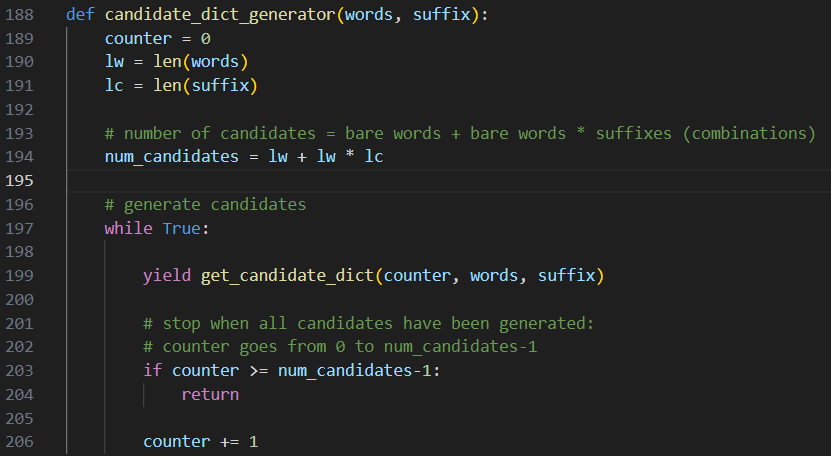
\includegraphics[width=0.8\columnwidth]{images/p1/q22.png}
				\caption{Screenshot of the modified function}
			\end{figure}
			
		\end{answer}
		
		\item (5 pts) What kind of passwords are recovered and for which users compared to Problem 0? Add a screenshot of your terminal output showing the answer. How long would it take to recover the same passwords using the bruteforce attack (Problem 0)? (Justify your answer.)
		
		\begin{answer}
			
			When comparing with the password recovered from the bruteforce attack, dictionary attack has been able to recover longer passwords for the user, James, John and David.
			
			\begin{table}[h]
				\centering
				\begin{tabular}{|l|l|}
					\hline
					\textbf{User} & \textbf{Password} \\ \hline
					James & mountain5 \\ \hline
					Robert & hat \\ \hline
					John & doughnut\# \\ \hline
					David & catcher@ \\ \hline
					Susan & pen \\ \hline
					Daniel & day2 \\ \hline
					Judy & toy \\ \hline
				\end{tabular}
				\caption{Recovered Passwords}
			\end{table}
		\begin{itemize}
			\item Time for the attack = 115.4 seconds
			\item Speed of the attack = 75130.7 hashes per second
			\item Attack success rate: 70\%
		\end{itemize}
			
				\begin{figure}[h]
				\centering
				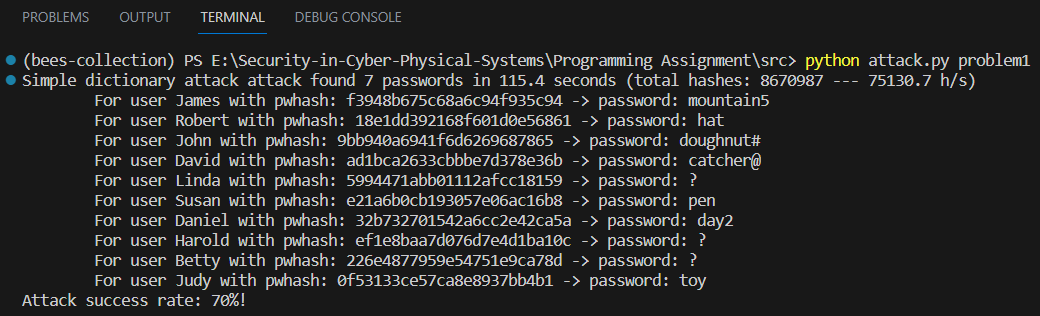
\includegraphics[width=0.7\columnwidth]{images/p1/q21.png}
				\caption{Output of the {\tt python attack.py problem1}}
			\end{figure}
			
						
			
			The longest recovered password has $l=9$ characters and they contain special characters from the list (defined in the program) in addition to the alphabet characters, therefore in total we have 26 + 36 possibilities per location in the password.\\
			
			Total number of possible passwords say $P$,
			
			\[
			P = \frac{62^{l+1}-1}{61} = \frac{62^{9+1}-1}{61} \approx 1.38 \times 10^{16}
			\]
			
			Average speed of the attack (this changes runtime-to-runtime and depending on the specifications of the machine used) therefore assume it to be $S = 60 \times 10^{3}$ hashes per second (an approximate value to the value that observed previously in problem0).\\
			
			Therefore approximate time in years say $Y$,
			
			\[
			Y = \frac{1.38 \times 10^{16}}{60 \times 10^{3}} \times \frac{1}{365 \times 24 \times 60 \times 60} \approx 7293.25 ~years 
			\]
			
			Brute force attack is not possible on this kind of passwords.
			
		\end{answer}
		
	\end{enumerate}
	
	\newpage
	\section*{Problem 2: Building a Rainbow table ({26 pts})}
	%
	
	In this problem, you will perform a Rainbow table attack against the same list of stolen password hashes (\texttt{data/simple-dbdump.json}). You will implement (part) of the password lookup rainbow table operation \texttt{lookup\_rainbow}() in \texttt{rainbow.py}. The code to build the rainbow table (\texttt{build\_rainbow}()) is provided. It will be useful to carefully read the code of \texttt{build\_rainbow}() and \texttt{test\_rainbow\_attack}() (in \texttt{attack.py}).
	
	Use the following to perform the attack:
	%
	\begin{Verbatim}
		python attack.py problem2
	\end{Verbatim}
	%
	
	%
	\begin{enumerate}
		
		\item (2 pts) How do rainbow tables differ from hash-reduce chains? Illustrate with an example.
		
		\begin{answer}
			
			In below illustrations, si, hi, pi and ei stands for start, hash, plaintext and end values respectively.\\
			
			Hash-reduce chains use the same reduce function (R) throughout the chain. This leads to potential merging of some hash-reduce chains as the reduce functions may not be collision resistant. 
			
			\begin{verbatim}
				s1 --H--> h1 --R--> p1 --H--> h2 --R--> e1
				s2 --H--> h3 --R--> p2 --H--> h4 --R--> e2
				s3 --H--> h5 --R--> p3 --H--> h6 --R--> e3				
			\end{verbatim}
			
			Rainbow tables solves this problem by using different reduce functions, k number of different reduce functions, in a chain of length k. In this case a collisions is only posible if chains hit the same value at the same iteration.  
			
			\begin{verbatim}
				s1 --H--> h1 --R1--> p4 --H--> h7 --R2--> e4
				s2 --H--> h3 --R1--> p5 --H--> h8 --R2--> e5
				s3 --H--> h5 --R1--> p6 --H--> h9 --R2--> e6								
			\end{verbatim}
			
		\end{answer}
		
		\item (2 pts) Briefly explain how you determine the length of a chain and the number of chains in a rainbow table. 
		
		\begin{answer}
		The length of a chain and the number of chains in a rainbow table represent a trade-off between the time and memory required to launch an attack. The more chains there are, the more disk space is required. The shorter the length of chain, faster the attack.	Therefore the values must be determined considering the available computing resources.
		\end{answer}
		
		\item (3 pts) How can you select different reduce functions to be used in different stages of the rainbow table?
		
		\begin{answer}
			`Different' reduce functions not necessarily mean that they are completely different set of function implementations. Most of the time it is the same reduce function whose output made depend on the iteration (location) of the chain. The iteration is also passed as an argument to the reduce function, which makes sure the same hash does not produce the same reduce value if the iteration is different.
		\end{answer}
		\pagebreak
		\item (16 pts) Complete the implementation of the rainbow table attack: \texttt{lookup\_rainbow}()! Test your implementation thoroughly. Your attack should recover the same kind of passwords as for Problem~0. Add screenshots of your terminal output showing the answer and the function implementation.
		
		\begin{answer}
			\begin{itemize}
				\item Time for the attack = 57.0 seconds
				\item Speed of the attack = 28058.5 h/s for rainbow-table building, 367.0 h/s for the attack
				\item Attack success rate: 20\%
			\end{itemize}
			
			\begin{figure}[H]
				\centering
				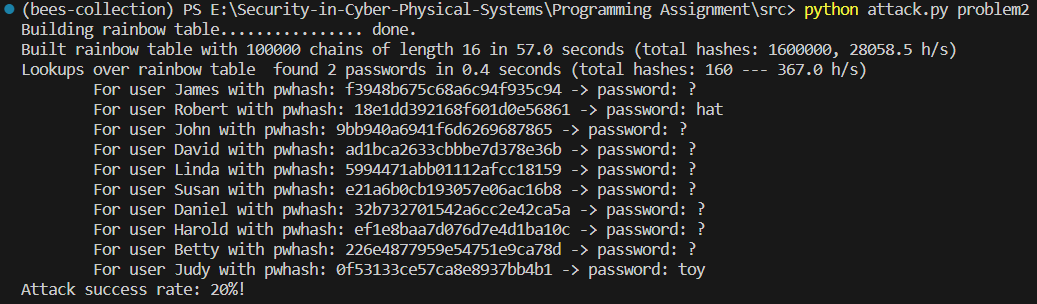
\includegraphics[width=0.7\columnwidth]{images/p2/q41.png}
				\caption{Output of the {\tt python attack.py problem2}}
			\end{figure}
		
			\begin{figure}[H]
				\centering
				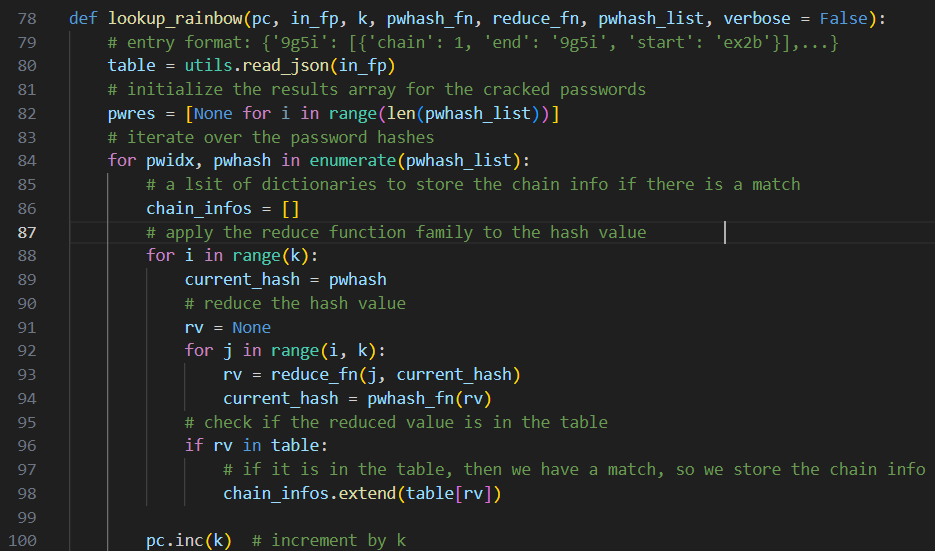
\includegraphics[width=0.7\columnwidth]{images/p2/q42.png}
				\caption{Implementation of the part 1 of \texttt{lookup\_rainbow}() function}
				\label{rainbow_lookup_1}
			\end{figure}
		
			\begin{figure}[H]
				\centering
				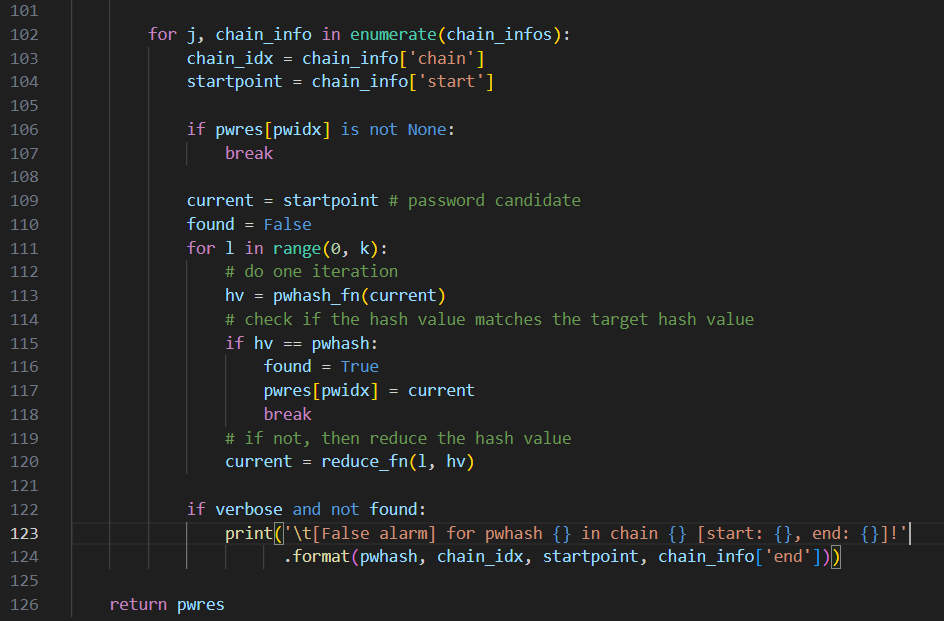
\includegraphics[width=0.7\columnwidth]{images/p2/q43.png}
				\caption{Implementation of the part 2 of \texttt{lookup\_rainbow}() function}
				\label{rainbow_lookup_2}
			\end{figure}
		
			
		\end{answer}
		
		\item (3 pts) What is a false alarm? Explain why it occurs and what we can do to minimize false alarms in rainbow tables.
		
		\begin{answer}
			
			False alarms are instances,\\
			1. We get an end point that is available in the rainbow table through reduce-hash procedure for the hash of a given password, \\
			2. However when we reconstruct the chain using the starting point of the corresponding end point, we do not hit the required hash of the given password.\\
			
			The reason for this is, \textbf{reduce functions are not collision resistant and different hashes can reduce to the same value}. 
			
		\end{answer}
		
	\end{enumerate}
	
	\newpage
	\section*{Problem 3: Understanding Rainbow tables (32 pts)}
	%
	
	In this problem, you will run the Rainbow table attack on a larger database of stolen password hashes (\texttt{data/complex-dbdump.json}). Unlike for previous problems, in this step all passwords consist of 4 alphanumeric characters --- lowercase only.
	
	Use the following command to run the attack:
	%
	\begin{Verbatim}
		python attack.py problem3
	\end{Verbatim}
	%
	
	Let $n$ denote the total number of possible passwords, $m$ denote the number of chains in the rainbow table, and $k$ denote the length of each chain.
	
	\begin{enumerate}
		\item (3 pts) What is the success rate of the attack (percentage of passwords recovered)? Why is it not 100\%?
		
		\begin{answer}
			
			Success rate = 52\%\\
			
			Success of a rainbow table attack depends on several factors such as the number of chains built and the length of a chain. If he number of unique starting points of chains is limited (at most 100,000 in this case), the password space that this attack can explore is less that the actual password space which is $36^4$.
			
			\begin{figure}[H]
				\centering
				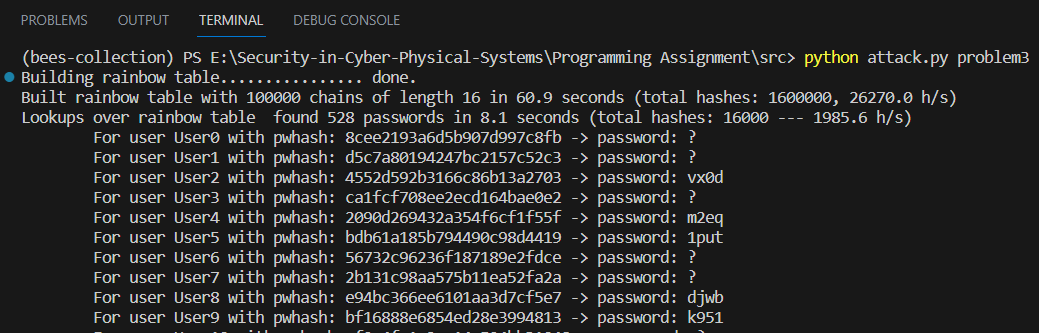
\includegraphics[width=0.7\columnwidth]{images/p3/q11.png}
				\caption{Launching the attack using the command {\tt python attack.py problem2}}
			\end{figure}
		
			\begin{figure}[H]
				\centering
				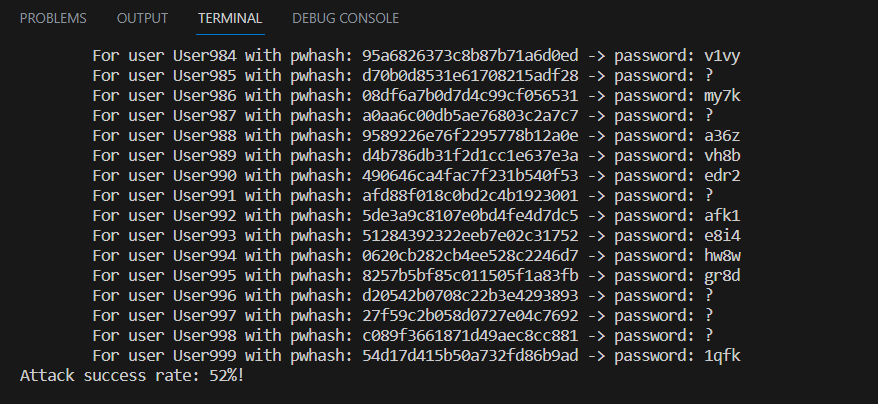
\includegraphics[width=0.7\columnwidth]{images/p3/q12.png}
				\caption{Output of the {\tt python attack.py problem2}}
			\end{figure}
			
		\end{answer}
		
		\item (4 pts) [Experimental] Keeping $m \cdot k$ constant, run the attack with $m = 25000$, $50000$, $100000$, $200000$, $400000$ and $k = 64, 32, 16, 8, 4$. (You can modify $m$ and $k$ in the \texttt{main}() function of \texttt{attack.py}.) 
		
		Record the success rate of the attack ($p$) and write it in the table below.
		
		\begin{answer}
			
			%% TODO: Write your answer here.	
			\begin{center}
				\begin{tabular}{|l|c|c|c|c|c|}
					\hline
					$m$ & 25000 & 50000 & 100000 & 200000 & 400000 \\ \hline
					$k$ & 64 & 32    & 16      & 8      & 4      \\ \hline \hline
					$p$ & 54\% & 53\%  &  52\%  & 56\%  &  55\%   \\ \hline
				\end{tabular}	
			\end{center}	
			
		\end{answer}
		
		\item (6 pts) Consider the case $k=1$. Observe experimentally that the success rate of the attack is lower than $\frac{m \cdot k}{n}$. Why is that?  To fix it, change the implementation of \texttt{build\_rainbow}() to ensure that each chain gets a unique startpoint. (Be careful to ensure that \texttt{build\_rainbow}() always terminates no matter the values of $n$, $m$, and $k$.)
		
		\begin{answer}
			
			Success rate for k = 1, is 60\%\\
			
			Note that, unlike for previous problems, in this step all passwords consist of 4 alphanumeric characters --- lowercase only, therefore total number of passwords $n = 36^4$.\\
			
			Expected success rate = $\frac{m \cdot k}{n} = \frac{1600000 \cdot 1}{36^4} = 95.26\% $\\
			
			A possible reason for this experimental success rate to be lower than the expected success rate is that, \textbf{start values of chains (password candidates) are randomly generated. Therefore, all possible passwords are not guaranteed to be captured during the table creation}. That means there can be chins with the same starting value.
			
			\begin{figure}[H]
				\centering
				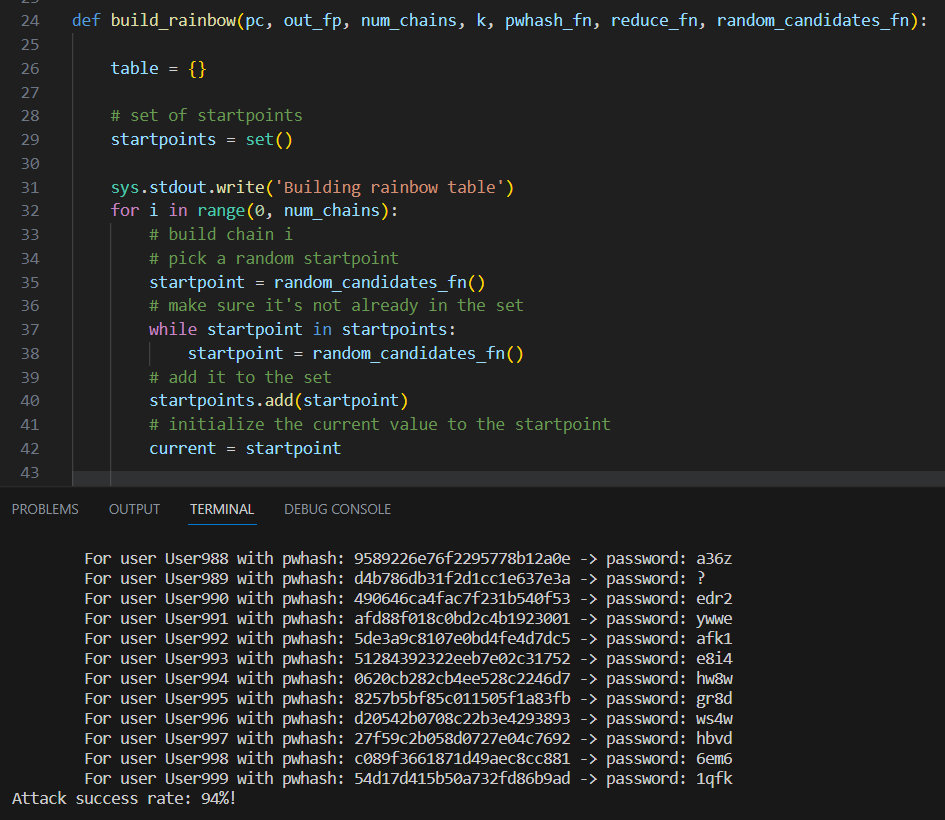
\includegraphics[width=0.7\columnwidth]{images/p3/q32.png}
				\caption{Modifications to make sure there are no duplicate start points}
				\label{p3q3}
			\end{figure}
			
			As illustrated in the Figure \ref{p3q3}, once we avoid the duplicate start points the success rate is 94\%. 
		\end{answer}
		
		\item (4 pts) [Theory] Explain the difference between hash and reduce functions and give 3 examples of possible reduce functions.
		
		\begin{answer}
			
			A hash function is a mathematical function which converts a given input message to a fixed-length string of bytes. The resultant representation is unique for a given input and small change in the input can cause a drastic change in the output (avalanche effect). In addition a hash functions are, 1. pre-image resistance, 2. second pre-image resistance and collision resistance.\\
			
			In contrast, reduce function is not an actual reverse of a hash value. It takes in a hash value and maps it to a value in the space of possible passwords through some mechanism. This mechanism yields a unique value for a given hash. However, they are not collision resistant, meaning two different hash values can map to the same value. Possible examples of reduce functions are given below.
			\begin{itemize}
				\item \textbf{Truncation}: truncates the hash value to a fixed length and maps it to a value in the password space.
				\item \textbf{Arithmetic operations}: performs arithmetic operations like modulo, integer division on the hash value or variant of it  to map it to a value in the password space. 
				\item \textbf{Bit extraction}:  extracts certain bits from the hash value and uses them as an index into the password space. 
			\end{itemize}
			
		\end{answer}
		
		\item $[$Theory$]$ Assume this password-cracking algorithm is implemented on a memory-limited system. Assume that a chain can be stored using 8 bytes (4 bytes for the startpoint, 4 bytes for the endpoint). Suppose we set $m$ and $k$ such that $n = m \cdot k$. Consider the system can compute 1000 hashes per second and 1000 reduction functions per second. (Assume time taken for other instructions is negligible when compared with hashing and reduction).
		
		\begin{enumerate}
			
			\item (2 pts) What is the amount of memory required to store the rainbow table?
			
			\begin{answer}
				
				Memory required = Memory per chain $\times$ Number of chains = 8 Bytes $\times$ $m$ = $8m~ Bytes$
				
			\end{answer}
			
			\item (3 pts) What is the expected computational complexity of a lookup?
			
			\begin{answer}
				
				Please note that, when calculating the time complexity of the lookup for a single password, the actual implementation of the function {\tt lookup\_rainbow()}  is used.
				
				It consists of two main phases,
				
				\begin{enumerate}
					\item \textbf{Finding the chains which can potentially include the password.}\\
					
					This part of the function is shown in the Figure \ref{rainbow_lookup_1}. It consists of one nested for loop which computes hashing $+$ reducing, $\frac{k}{2}\times\left( k+1 \right)$ times. Finding a chain in the dictionary object has constant time complexity and therefore neglected.\\
					
					\item \textbf{Rebuilding the chains to find the password.}\\
					
					This part of the function is shown in the Figure \ref{rainbow_lookup_2}. It rebuilds the chain for each potential chain match and check whether the password is in a given chain. At most we can have $m$ potential chains (total chains) and  for each chain we have $k$ number of hashing $+$ reducing. Therefore this part of the function computes  hashing $+$ reducing, $m \times k$ times.
				\end{enumerate}
			
			Therefore the total time complexity of the entire lookup for a single password is,
			
			\[
			  O\left( \frac{k}{2}\times\left( k+1 \right) \right) + O\left( m \times k \right) = O\left( k^2 \right) + O\left( m.k \right)
			\]
			
			Since we keep the $n= m.k$ constant, The actual time complexity of the lookup is $O(k^2)$.
				
			\end{answer}
			
			\item (4 pts) Determine the optimum value for $k$ such that it uses the lowest memory space to store the rainbow table.
			
			\begin{answer}
				
				Memory required in Bytes = $8m$\\
				Replacing $m$ using the equation  $n = m \cdot k \rightarrow m = \frac{n}{k}$\\
				
				Memory = $8 \times \frac{n}{k}$\\
				
				As it can be seen to minimize the memory usage, we need to increase the chain length. However increasing $k$ will increase the time complexity of the lookup operation as proved in the previous problem. Therefore we need to select the largest possible $k$, which respects that constraint as well. Therefore, $k$ value becomes a trade-off, which must be calculated experimentally.
				
				
			\end{answer}
			
		\end{enumerate}
		
		\item (6 pts) [Experimental] Keeping $m \cdot k$ constant, run the attack for $m = 25000$, $50000$, $100000$, $200000$, $400000$ and $k = 64, 32, 16, 8, 4$. Plot the time for a lookup in each case. How does this compare to your answer to Problem 3, part 5(b)?
		
		\begin{answer}
			
			\begin{center}
				\begin{tabular}{|l|c|c|c|c|c|}
					\hline
					$m$ & 25000 & 50000 & 100000 & 200000 & 400000 \\ \hline
					$k$ & 64 & 32    & 16      & 8      & 4      \\ \hline \hline
					$p$ & 54\% & 53\%  &  53\%  & 57\%  &  58\%   \\ \hline
					$t/lookup$ &  0.11972 & 0.03027 &0.00837 & 0.00207& 0.00059\\ \hline
				\end{tabular}	
			\end{center}
		
		\begin{figure}[H]
			\centering
			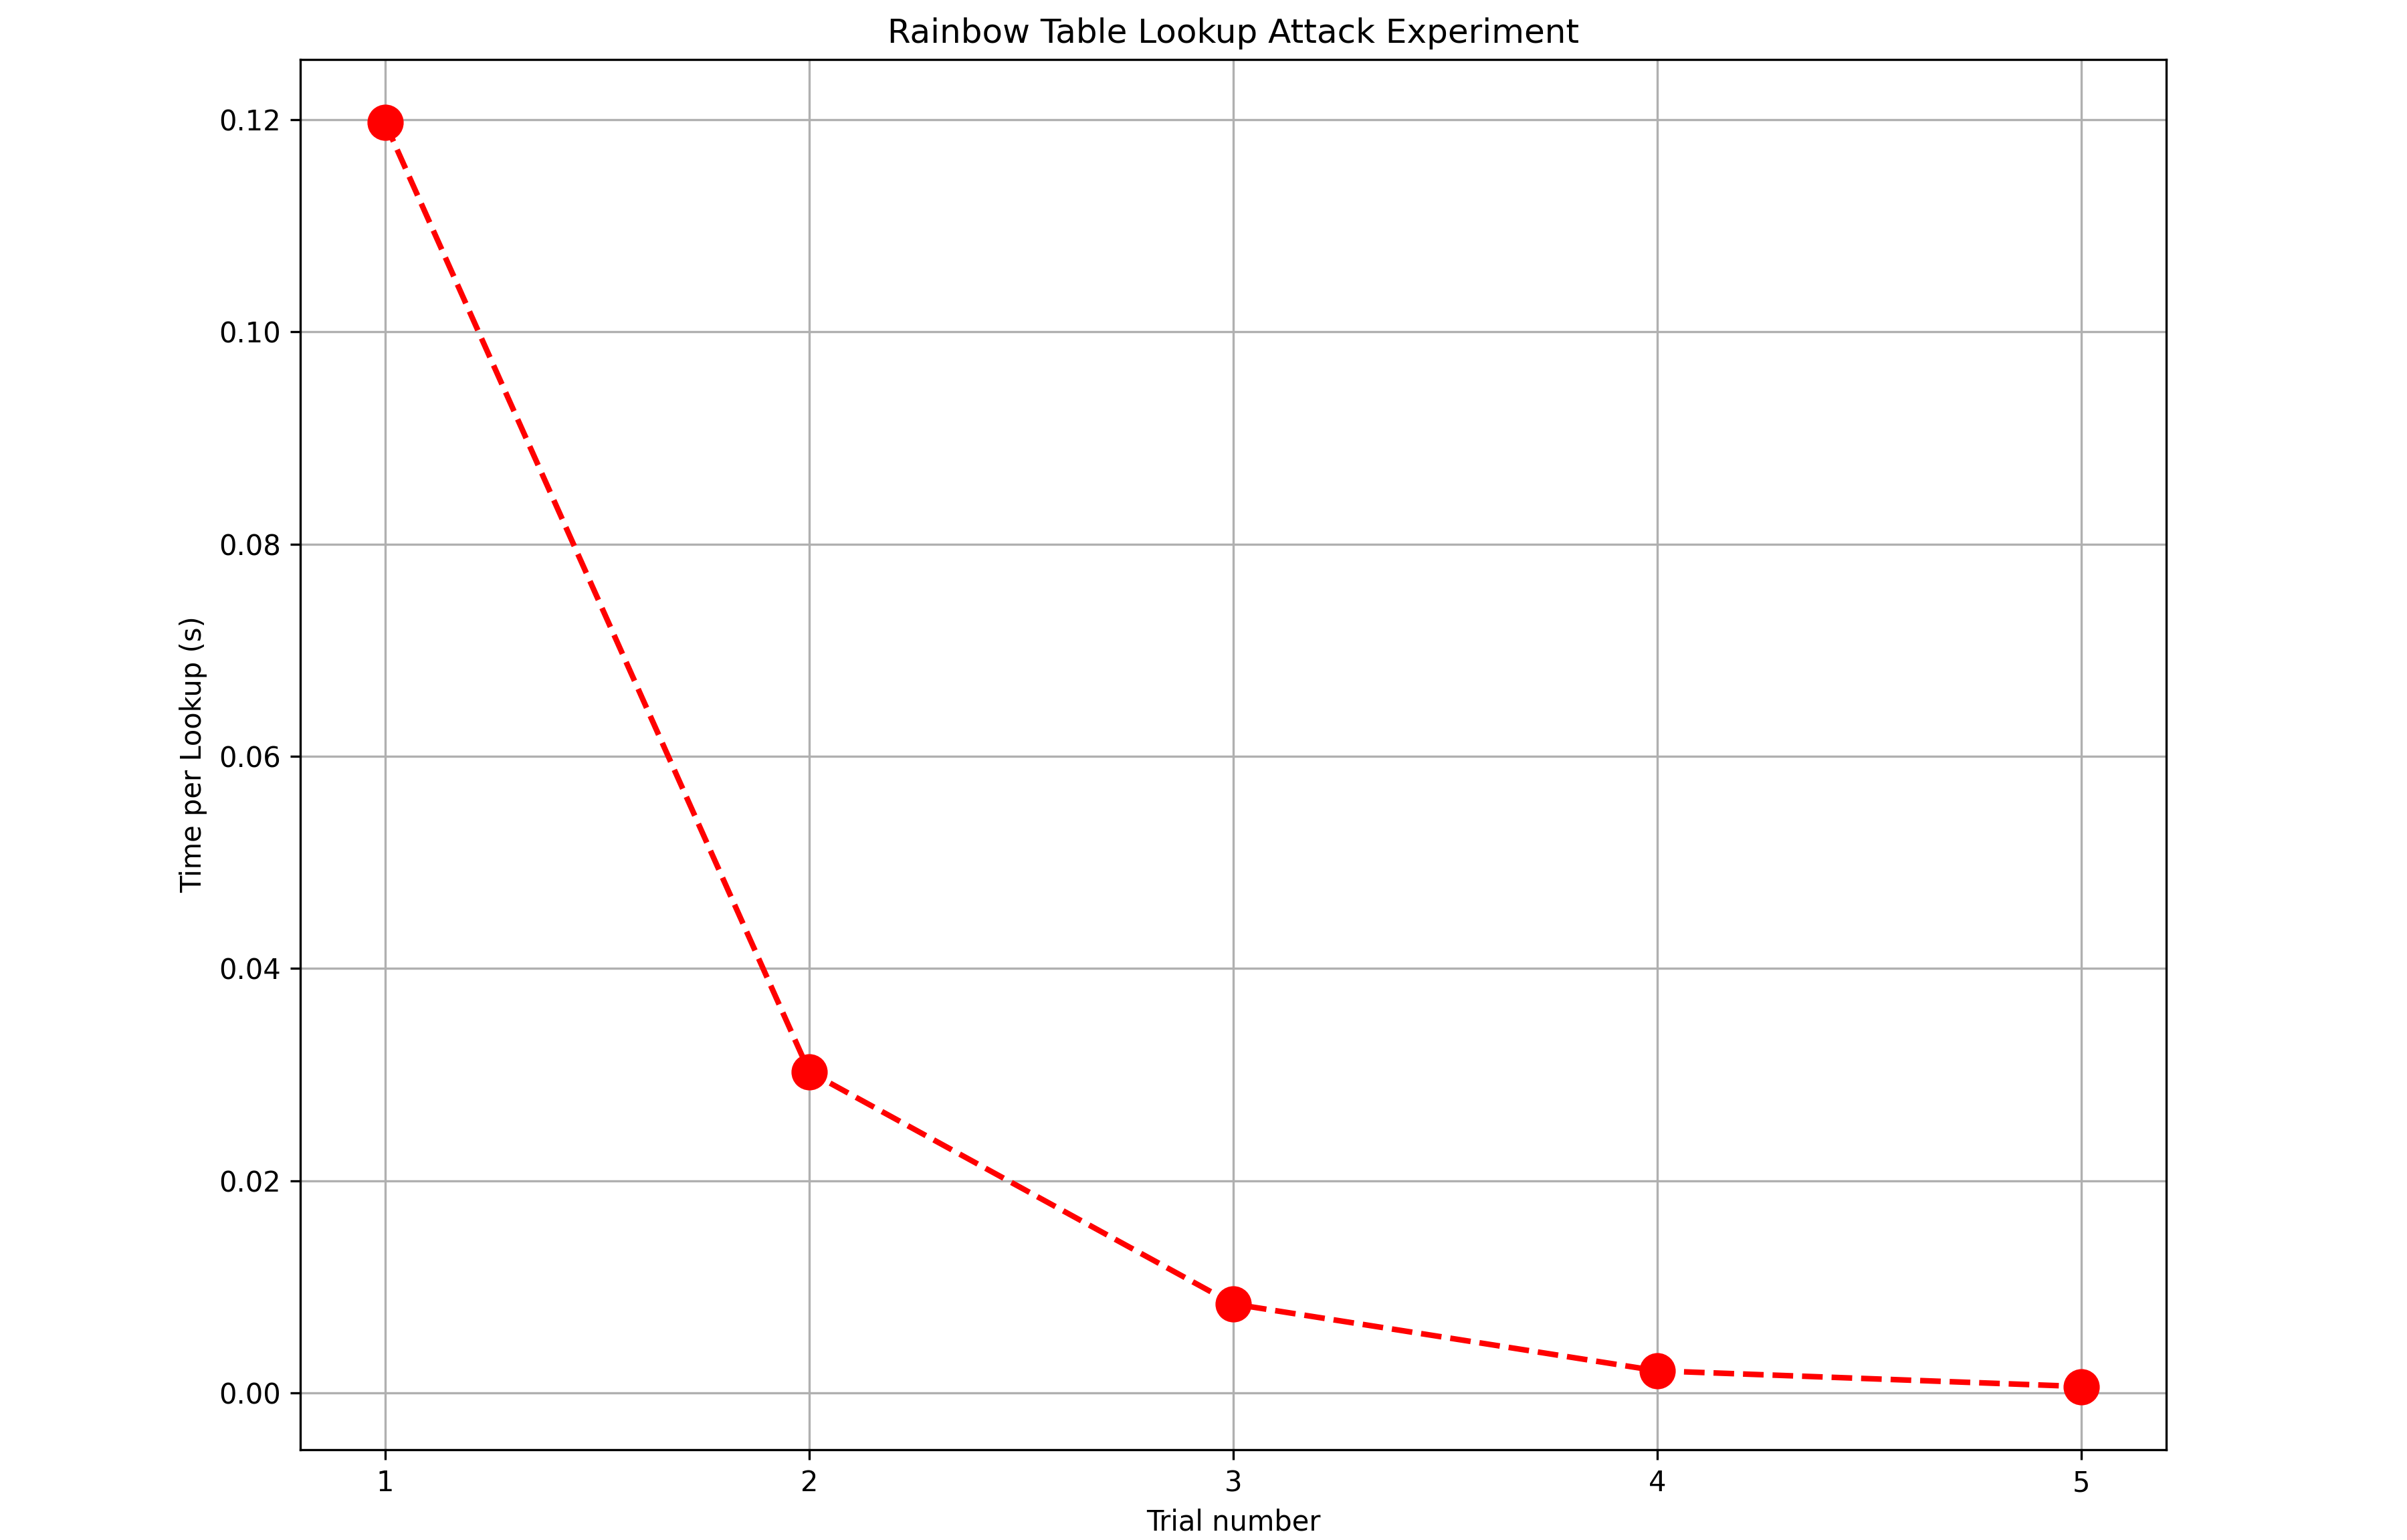
\includegraphics[width=0.6\columnwidth]{images/p3/plot.png}
			\caption{Plot of the time for a lookup in each case}
		\end{figure}
			
		 When this plot is compared with the  answer to Problem 3, part 5(b) the expected time complexity   $O(k^2)$ agrees with the experimental results. That is when the $k$ is decreased, the time for a lookup has reduced exponentially. 
			
		\end{answer}
		
	\end{enumerate}
	
	\newpage
	
	\section*{Problem 4: Bob's custom password hash (14 pts + [bonus] 10 pts)}
	%
	
	Your classmate Bob is in charge of the website of E-Club, ENTC. To implement authentication on the website, Bob (who has not taken EN4720) has decided to roll his own crypto. He has implemented a custom password hash function. Given a password $p$ of even length, $p$ is split into two parts of equal lengths $p_1$, $p_2$. The password hash is then computed as:
	\[ H_l(p_1) || H_l(p_2) || H_l^i(s || c) , \]
	where $s$ is a random salt, $c$ is a constant string, $i$ and $l$ are positive integers. Here: $H_l(x)$ denotes the first $l$ bytes of the hash of $x$. This password hash is implemented as \texttt{bobs\_custom\_pw\_hash}() in \texttt{crypto.py}.
	
	
	For this problem, you will implement your own attack against Bob's custom password hash scheme. For this you will use \texttt{data/bobX-dbdump.json} as database of password hashes.
	
	Use the following command to run your attack:
	%
	\begin{Verbatim}
		python attack.py problem4
	\end{Verbatim}
	%
	
	
	%
	\begin{enumerate}
		
		\item (2 pts) Is it a good idea to design your own crypto like Bob did in this case? Explain why or why not?
		
		\begin{answer}
			
			It is not advised to design your own crypto, especially if you are not an expert in the field of cryptography. 
			
			According to the Schneier's law ``Anyone, from the most clueless amateur to the best cryptographer, can create an 
			algorithm that he himself can't break.'' 
			
			Therefore the best option is to go for a publicly available well-established crypto which has undergone extensive scrutiny.
			
		\end{answer}
		
		\item (3 pts) Give your comments on the salting mechanism used by Bob in his custom crypto. Does his method serve the purpose of salting? Explain your answer.
		
		\begin{answer}
			
			To serve the purpose of making it harder to crack the password, \textbf{the salt must be concatenated with the password before hashing it}. 
			
			However, what Bob has done is meaningless. Because, \textbf{the two parts of the password and salt are hashed separately and then concatenated}. Still the real password is not contaminated by the salt. 
			
			Password can still be recovered by attacking only the 	$H_l(p_1) || H_l(p_2)$ part of the hash without considering the hash part coming from the salt.
			
		\end{answer}
		
		\item (3 pts)  Bob’s friend Alice says the splitting of the password into 2 equal parts and hashing them separately will make the life of an attacker difficult to launch a bruteforce attack. Do you agree with this statement? Give reasons.
		
		\begin{answer}
			
			Disagree with the statement.
			
			Splitting the password in to 2 equal parts, will not make the life of an attacker difficult to launch a bruteforce attack. Because now the length of the password has become half and possible size of the password space has reduced drastically. 
			
			As an example let's say password is 8 characters and lowercase alphanumeric.  
			\begin{itemize}
				\item If the password is not split, total possible passwords = $36^8$
				\item however, after splitting total possible passwords = $36^4$, and each part can be brute forced separately. This would be much faster than brute-forcing the entire password.
			\end{itemize}
			
		\end{answer}
		
		\item (3 pts)  Is it a good idea to use the first $l$ bytes of the hashes as in Bob's crypto? Explain your answer giving reasons.
		
		\begin{answer}
			
			It is a bad idea.
			
			One of the main properties of a hash value is its collision resistance, which makes it very difficult for an attacker to find two input values with the same hash. For this property to hold it hash should be of full length.
			
			However, considering the first $l$  bytes will reduce number of possible hashes, as now we do not need to consider the full hash length. This makes it easier for an attacker to find a collision.
						
		\end{answer}
		
		\item (3 pts) Suggest a suitable method to make this custom password hash scheme difficult to crack by the attackers.  
		
		\begin{answer}
			
			The fundamental weaknesses of Bob's password scheme are follows.
			\begin{itemize}
				\item Salt is not actually concatenated (applied) to the passwords; it is separate.
				\item Password has been split into two parts making it easy to brute force them separately.
				\item  Only the  first $l$ bytes of the hashes have been considered to build the final password hash. 
			\end{itemize}
			
			Hashing it again will not address this fundamental weaknesses. Therefore, in order to make the scheme stronger, we have to directly address the mentioned weaknesses by doing followings.
			
			\begin{itemize}
				\item Make it a requirement to have a minimum length (at least 8) to the bare password and add salt directly to the password parts to make the brute-forcing difficult. Eg. $p1 + s \geq 8 ~\&~ p2 + s \geq 8 $ will be a good choice.
				
				\item Increase the number of bytes ($l$) that we consider when building the password hash. This will make it more collision resistant.
			\end{itemize} 
			
		\end{answer}
		
		
		\item ([\textcolor{magenta}{bonus}] 10 pts) Implement the best attack you can think of. Place your code in the provided placeholders in \texttt{bobs\_custom\_pwhash\_attack}() (\texttt{attack.py}). You will be evaluated based on the performance of your attack on passwords of varying length. You can change the size of the targets passwords by changing the value of \texttt{pw\_length} in the \texttt{main()} function of \texttt{attack.py}.
		
		{\em Hint: the fastest attack is neither the naive bruteforce attack nor the one based on rainbow tables.}
		
		Explain how your attack works. How fast is it on passwords of length 4, 6, and 8?
		
		\begin{answer}
			
			Not implemented.
			
		\end{answer}
		
	\end{enumerate}
	
\end{document}
